
% 2 sadaļas, footeris, main content

Izstrādāto galaprojektu ir iespējams uzstartēt ar \emph{shell} skrptu projekta
pamatdirektorijā \texttt{./start.sh}.
Projektu uzstartējot, apmeklējot ar interneta pārlūkprogrammu saiti
\url{https://127.0.0.1:5001/}, atvērsies lapa, kāda attēlota \ref{img:whole-ui} attēlā.

\begin{figure}[H]
	\centering
	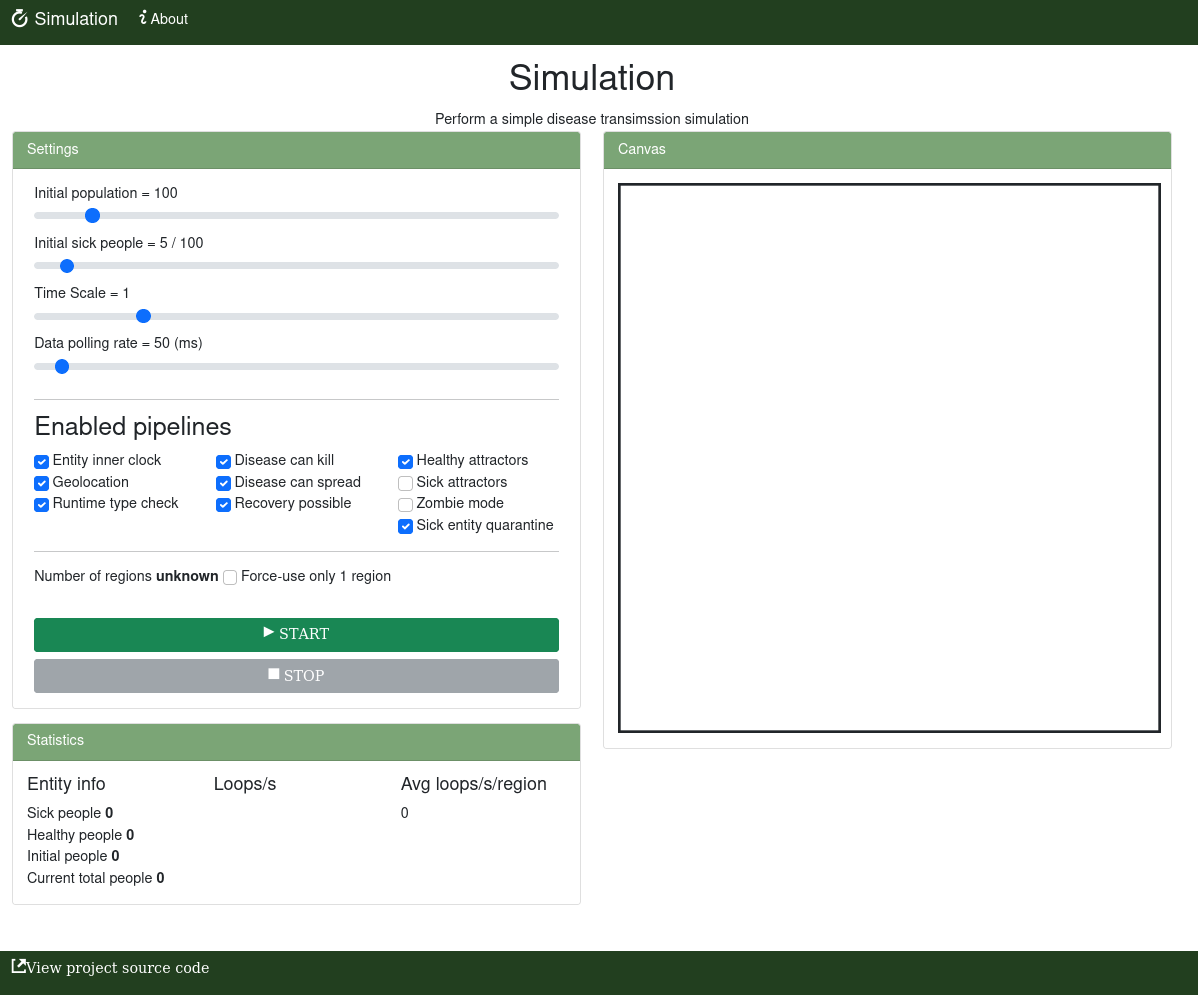
\includegraphics[scale=0.4]{images/ui-whole-page.png}
	\caption{Lietotāju saskarnes sākuma skats}
	\label{img:whole-ui}
\end{figure}

Lietotāju saskarne sastāv no divām lapām - pašas simulācijas (\ref{img:whole-ui}
att.) un ,,About" sadaļas (nav attēlots atskaitē).

% Settings panelis

,,Settings" panelis ir galvenā vieta saskarnē, kur ir iespējams veikt sekojošās darbības:

\begin{itemize}
    \item \emph{Pipeline} ieslēgšanu/izslēgšanu,
    \item populācijas skaita maiņu,
    \item slimo entītiju skaita maiņu,
    \item datu pieprasīšanas intervāla (\emph{polling rate}) maiņu,
    \item iespēja piespiedus kārtā izmantot tikai vienu \emph{Region} instanci
    \item Uzsākt/apstādināt simulāciju
\end{itemize}

% Canvas

\emph{Canvas} elements attēlo simulācijā esošos entītijus lietotājam. Ņemot vērā, ka
simulācijas plaknes izmēri nesakrīt ar pikseļu dimensijām lietotāju saskarnes
\emph{canvas} elementa izmēriem, tad katrs punkts arī tiek normalizēts jaunajās
(lietotājam redzamajās) dimensijās. Zināmas problēmas gan rodas gadījumos, kur
ir liels entītiju skaits -- \emph{canvas 2d context} nespēj pietiekami ātri
uzzīmēt lielo elementu skaitu, rodas vizuāli artefakti. \emph{Canvas} elementus
ar dažādiem simulāciajs stāvokļiem dažādās stadijās var apskatīt \ref{img:canvas-show-off} attēlā.

\begin{figure}[H]%
    \centering
    \subfloat
        [\centering Karantīna tiek ievērota (\emph{Healthy attractors} ieslēgts)]
        {{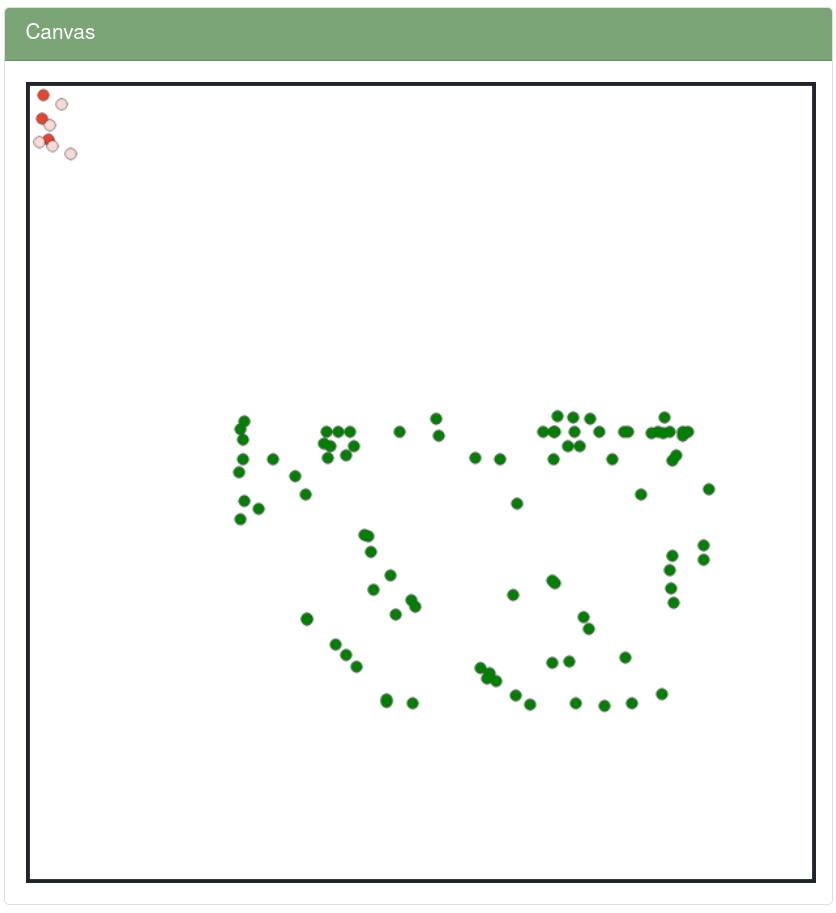
\includegraphics[width=.3\linewidth]{images/quarantine.png} }}%
    \qquad
    \subfloat
        [\centering Slimība izplatās, ja karantīna netiek ievērota]
        {{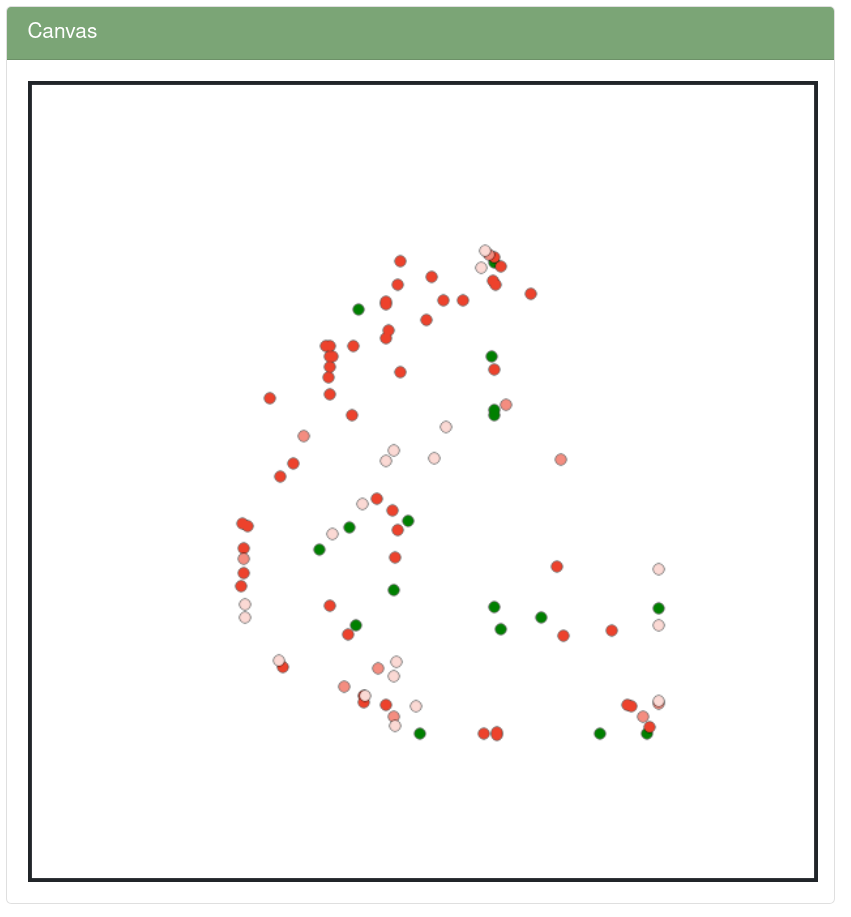
\includegraphics[width=.3\linewidth]{images/sickness-spreads.png} }}%
    \subfloat
        [\centering Atraktori ir izslēgti, ieslēgts \emph{Zombie mode}]
        {{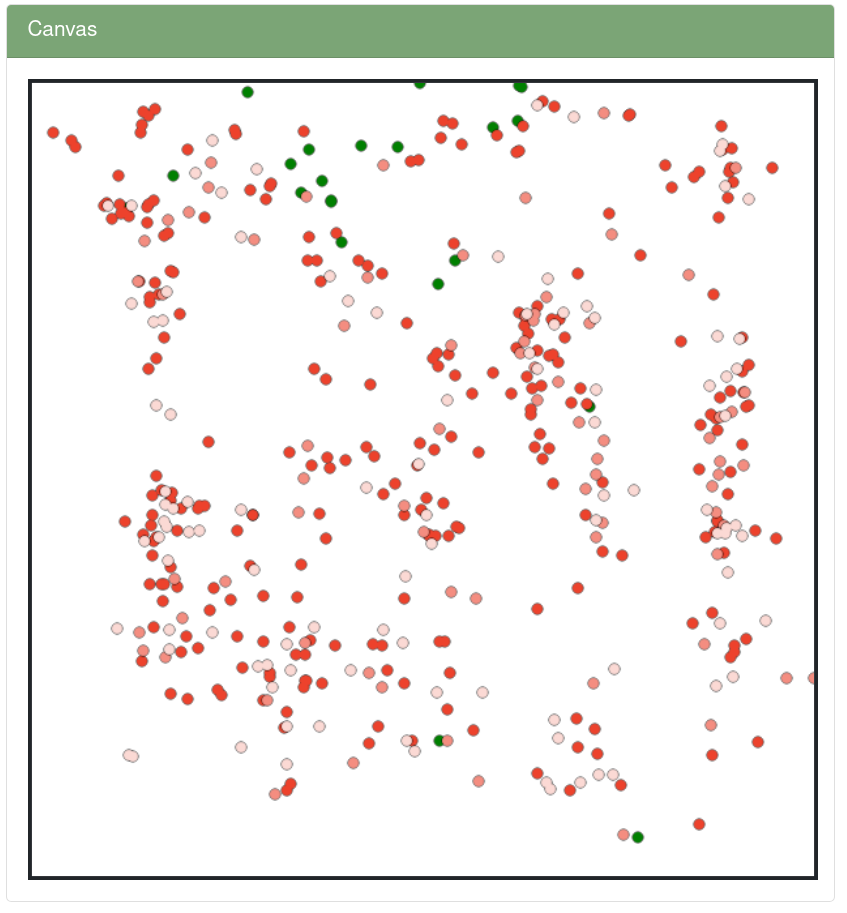
\includegraphics[width=.3\linewidth]{images/zombiemode-1.png} }}%
    \qquad
    \subfloat
    [\centering Ilgtermiņā turot ieslēgtu \emph{Zombie mode}, var redzet \emph{Region} sadalījumu]
        {{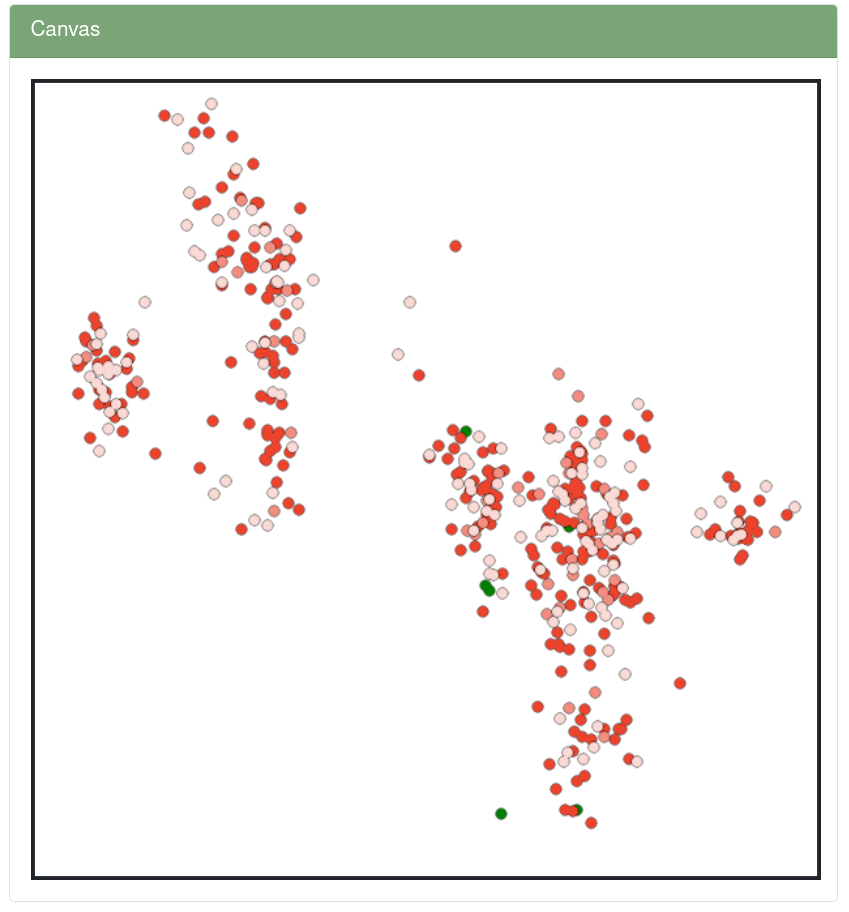
\includegraphics[width=.5\linewidth]{images/zombiemode-2.png} }}%
    \caption{Dažādu simulāciajs stāvokļu viuzalizācija}%
    \label{img:canvas-show-off}%
\end{figure}

% Statistics



% Screenshot no htop ka izpildās uz pilnu slodzi
